\documentclass[hidelinks]{report}

\usepackage{graphicx}
\usepackage{times}
\usepackage{plain}
\usepackage[plainpages=false]{hyperref}
\usepackage{courier}
\usepackage{caption}

% To force figures to appear after text(along with [H] option)
\usepackage{float}

% To apply linespacing to some content
\usepackage{setspace}

% To show commands, code snippets
\usepackage{listings}

% To use checkmark (tick symbol)
\usepackage{amssymb}

\graphicspath{ {images/pdf/} }

\pagestyle{plain}

\fontfamily{Times}
\selectfont

\setlength{\textwidth}{6.5in}
\setlength{\textheight}{8.5in}
\setlength{\topmargin}{-0.25in}
\setlength{\oddsidemargin}{-0.00in}
\setlength{\evensidemargin}{-0.00in}

% To use multirow feature of latex tables
\usepackage{multirow}

% Using and defining own color
\usepackage{color}
\definecolor{mycol}{RGB}{52, 43, 41}

% Defining courier font usage syntax
\newcommand{\cf}[1] {
	\textbf{\texttt{#1}}
}

% Defining checkmark usage syntax
\newcommand{\T} {
	\checkmark
}

\begin{document}

%% Line spacing 1.5 applied
\setstretch{1.5}

\begin{center}
\section*{vEPC 1.0 Developer Manual}
\end{center}

\paragraph*{NOTE:}

This manual is split into two parts. Part-1 deals with the design and implementation details of various software modules that were developed as part of our vEPC. Part-2 deals with a high level description of individual source code files (\cf{.cpp/.h}). Please read the \cf{user\_manual.pdf} under \cf{doc} folder for instructions on experimenting with our vEPC.

\begin{center}

\subsection*{PART-1 \\ Design and Implementation}

\end{center}

We have designed and implemented various EPC modules (MME, HSS, SGW, PGW) along with a RAN simulator and a Sink node. The whole setup can be called as a NFV-based LTE EPC and its sketch is shown in figure~\ref{nfv_lte_epc}. RAN simulator is used for the purpose of generating traffic to our EPC. Sink module is used to receive the generated uplink traffic and send back acknowledgement data as downlink traffic.

\begin{figure}[H]

\centering
\includegraphics[scale=0.4]{nfv_lte_epc}
\caption{NFV-based LTE EPC system.}
\label{nfv_lte_epc}

\end{figure}

\subsection*{Virtualized EPC}

In the Virtualized EPC (Figure~\ref{nfv_lte_epc}), the core network functions of the EPC (MME, HSS, SGW, PGW) are built as software modules, and are run on VMs hosted on a cloud. The design and implementation details of the Virtualized EPC are given in the following sections.

\subsection*{Design}

The overall design of the system is based on client-server paradigm, where the server is multithreaded to satisfy concurrent client requests. This effectively captures all necessary functionalities involved in a typical EPC. Standard communication protocol stacks prescribed by 3G Partnership Project (3GPP) are used across the implemented system, as shown in figure~\ref{nfv_lte_epc}. We have modified the formats of the S1AP and diameter protocols slightly for ease of implementation; the rest of our implementation faithfully follows the standards. Each of the EPC components (MME, SGW, PGW, HSS) are implemented as multithreaded servers that service requests (e.g., UE attach request) from the downstream nodes and send responses back. Note that every component acts as a server to the downstream node, and as a client to the upstream node in the chain of VNF components traversed by a request. The MME application module employs Stream Control Transmission Protocol (SCTP) for its communication with eNodeB and HSS. For ease of implementation, we did not use the multi-streaming feature of SCTP. The EPC gateways are built around a multithreaded UDP server, because the protocol stack of the gateways uses UDP to communicate with the other components. Below, we elaborate on our multithreaded server architectures.

\paragraph*{Multithreaded SCTP Server architecture}

~\\ The SCTP server architecture consists of a single master thread and several worker threads, as shown in figure~\ref{sctp_arc}. The master thread communicates with each of the worker threads via a logical Unix pipe. The master thread listens for incoming client connections on a stream socket, and creates an additional socket file descriptor for every new SCTP client that is accepted. It then sends the new connection socket file descriptor to the worker threads. in a round-robin fashion, to balance load across all worker threads. The worker thread is responsible for servicing the request on the new connection, through all the setups required to handle the request. For example, the worker thread in the MME must implement the various steps required to process an UE attach request, blocking for responses at each stage from the other nodes. The workers threads use the event-driven select mechanism to multiplex the multiple requests being handled by each of them concurrently. The number of worker threads in this architecture can be sized to fully utilize all the processing cores of the VM.

\begin{figure}[h]

\centering
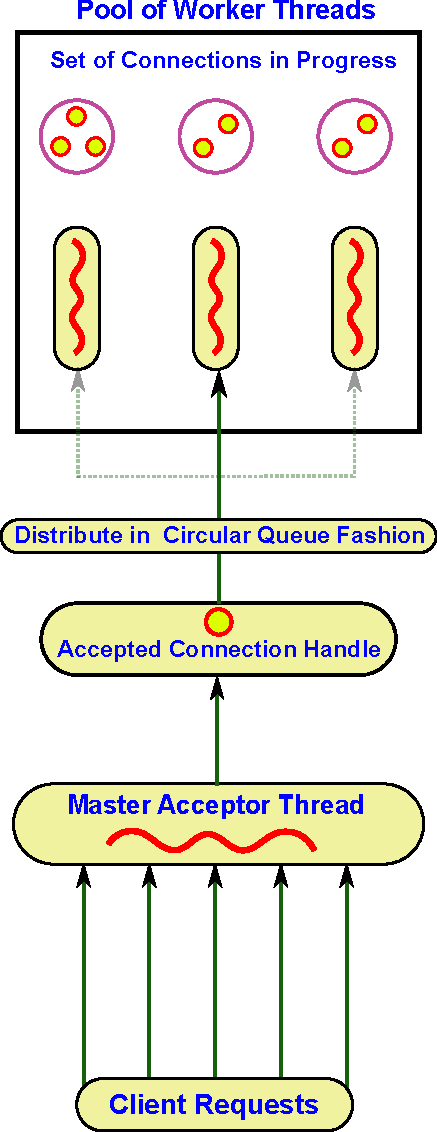
\includegraphics[scale=0.5]{sctp_arc}
\caption{Multithreaded SCTP Server architecture.}
\label{sctp_arc}

\end{figure}

\paragraph*{Multithreaded UDP Server architecture}

~\\ The UDP server architecture consists of a single datagram socket being serviced by multiple server threads. All server threads try to read a UDP packet from the common shared socket. The thread that succeeds in reading the packet is responsible for processing the request and sending a response back to the downstream node. Figure~\ref{udp_arc} shows the multithreaded UDP architecture. By fixing a suitable number of server threads in proportion to the number of system cores, this architecture provides good performance and scalability. 

\begin{figure}[h]

\centering
\includegraphics[scale=0.5]{udp_arc}
\caption{Multithreaded UDP Server architecture.}
\label{udp_arc}

\end{figure}

~\\
In both the server architectures, a global data structure is used by the threads to store/retrieve necessary connection data and state. This data structure is protected by locks to prevent concurrent inconsistent access by the multiple threads. As part of future work, we plan to redesign our system using lock-free data structures to eliminate contention among the threads for shared data structures.

\subsection*{Implementation}

The overall implementation is based on the object-oriented paradigm, where each EPC entity employs either a server or a client object on each one of its ports. These ports correspond to the standard interfaces prescribed by 3GPP, and are listed as follows: S1-MME, S1-U, S11, S5-C, S5-U, S6a and SGi. The object and the underlying protocol being employed are dependent on the standard interface port under consideration. Control and data communication happen through these objects sending requests/responses among various entities in the system. A short description of each of the EPC entities is given below.

\paragraph*{Mobility Management Entity}

~\\ The software module that governs MME communicates with other system modules on three different ports corresponding to three different standard interfaces: S1-MME, S6a and S11. On S1-MME interface port, it uses a SCTP server object to communicate with eNodeB for UE session/bearer set up and tear down. On S6a interface port, it uses a SCTP client object to communicate with HSS for fetching UE related information and UE location update. On S11 interface port, it uses a UDP client object to communicate with SGW for session/bearer related procedures. A global hash map is maintained for usage across all communication to store connection and state information related to UEs. The hash map is accessed/updated upon subsequent requests/responses from the UEs, HSS and SGW.

\paragraph*{Home Subscriber Server}

~\\ The software module for HSS uses a MySQL object for database related operations and a SCTP client object for communication with MME on its S6a interface port. Several table instances are created in MySQL database for storing UE related information such as authentication,  subscription profile and location tracking. All MME queries are responded with corresponding information fetched and processed from the database.

\paragraph*{Serving Gateway}

~\\ The software module for SGW handles control plane communication with MME and PGW on S11 and S5-C interface ports respectively. On S11 interace port, it uses a UDP server object and on S5-C interface port, it uses a UDP client object. On the other hand, it handles data plane communication with eNodeB and PGW on S1-U and S5-U interface ports respectively. On S1-U interface, it uses a UDP server uplink object and a UDP client downlink object. On S5-U interface, it uses a UDP server downlink object and a UDP client uplink object. As in the case of MME entity, it also uses a hash map for storing UE context information.

\paragraph*{Packet Data Network Gateway}

~\\ The software module for PGW handles control plane communication with SGW on S5-C interface port through a UDP server object. It handles data plane communcation with SGW and Sink on S5-U and SGi interface ports respectively. On S5-U interface, it uses a UDP server uplink object and a UDP client downlink object. On SGi interface, it uses a UDP server downlink object and a UDP client uplink object. UE related information are accessed/updated in a separate hash map. A separate IP table map is also used to assign a static IP address for each UE being connected to the EPC.

\subsection*{Radio Access Network (RAN) Simulator}

We also built a RAN simulator that combines the functionalities of UE and eNodeB, in order to generate control and data traffic to our EPC. We do not implement the radio procedures that take place between UE and eNodeB in the RAN simulator, and focus only on the traffic that is seen by the EPC. The RAN simulator spawns multiple threads and creates a RAN object for each thread, which in turn handles control plane and data plane communication with MME and SGW respectively. For the process of tunneling during UE data transfer, separate threads are spawned to monitor and fetch UE packets coming from the kernel stack.  For control plane communication, a SCTP client object is used on S1-MME interface port for UE session/bearer set up and tear down procedures. For data plane communication, separate UDP client/server objects are used on S1-U interface port for uplink/downlink data transfer. A global array of RAN contexts is used for  maintaining all information related to both UEs and eNodeBs.

\subsection*{Sink Module}

A separate sink module to represent the PDN server has also been implemented. It is used to receive the generated uplink traffic and send back the acknowledgement data as downlink traffic.  Much like in the case of RAN simulator, multiple sink objects are created, each in its own thread. Each sink object uses separate UDP server/client objects on SGi interface for uplink/downlink data transfer with PGW.

\subsection*{Handling LTE procedures}

We now present the details involved in handling the basic LTE procedures using our NFV-based LTE EPC system. The various procedures that are evaluated include attach, detach and uplink/downlink data transfer. We found these procedures to be sufficient to cover the control and data functionalities at all nodes. We are in the process of implementing handover and other features in our code. As stated earlier, the functionalities of UE and eNodeB are combined into a single RAN entity and hence, UE and eNodeB both denote the RAN object in all our further description. Also packet type identification is done based on the underlying interface and protocol header fields. An illustration of the above mentioned procedures is given in the following sections.

\subsection*{UE Attach}
Figures~\ref{nfv_nas_conn} and ~\ref{nfv_eps_conn} show the control flow diagram of a UE attach procedure. This procedure includes several subprocedures that are listed as follows (in sequence): Authentication, NAS Security setup, Location update, Evolved Packet System (EPS) Session/Bearer setup. A brief overview of these subprocedures is given below.

\begin{figure}[h]

\centering
\includegraphics[scale=0.5]{nfv_nas_conn}
\caption{Attach Implementation: NAS Signaling Connection Setup.}
\label{nfv_nas_conn}

\end{figure}

\begin{figure}[h]

\centering
\includegraphics[scale=0.5]{nfv_eps_conn}
\caption{Attach Implementation: EPS Session/Bearer Setup.}
\label{nfv_eps_conn}

\end{figure}

\paragraph*{Authentication}

\begin{enumerate}

\item UE sends its key identifier (Internation Mobile Subscriber Identity (IMSI)) along with its other network/session/bearer related parameters to the MME.

\item On receiving the initial attach request from the UE, the MME verifies that it is a new service request and starts its authentication procedure by requesting HSS for UE related data.

\item Once HSS processes the datagram and sends back the results, the MME would reply authentication parameters to the UE. It also stores the expected result in its global hash map for this UE.

\item UE on receiving the authentication parameters, calculates the authentication result with its key and performs network authentication. It also sends the result back to the MME. To verify authentication, the MME fetches the expected result from the global hash map and then compares this with the result it received from the UE. If the results match, MME sends \textbf{OK} response and if it does not match, it sends \textbf{FAILURE} response. This ends the process of authentication.

\end{enumerate}

\paragraph*{NAS Security setup}

\begin{enumerate}

\item After successful authentication between UE and MME, MME sends UE the security context (NAS encryption and integrity algorithms, other network, key parameters). This message is sent along with Hashed Message Authentication Code (HMAC).

\item The UE derives the corresponding keys from the security context sent by the MME. Then the UE verifies the HMAC with the derived security key for integrity check. After successful verification, it sends a positive response that is encrypted and hashed (HMAC digest). 

\item Once the MME decrypts and verifies the HMAC positively, the NAS security setup becomes successful. 

\item After successful NAS security setup, any data that is communicated between UE and MME is always encrypted and hashed.

\end{enumerate}

\paragraph*{Location update}

~\\ After successful security setup, the MME updates the location of the UE in HSS for future references. This becomes useful during paging of service request procedure after S1 connection release.

\begin{itemize}

\item During location update, the MME sends the Tracking Area Identifier (TAI) of the UE's current location to the HSS for future references. At the end of location update procedure, NAS signaling connection has been established between UE and MME.

\end{itemize}

\paragraph*{EPS Session/Bearer setup}

~\\ During the EPS Session/Bearer setup, MME performs Create Session and Modify Session procedures as given below.

\begin{enumerate}

\item \textbf{Create Session}

\begin{enumerate}

\item The MME generates S11 MME Control TEID (CTEID) and sends it along with UE context to the SGW. 

\item The SGW stores the TEID and UE context received from MME. It then creates a bearer for this UE and generates TEIDs for S11 SGW, S1-U uplink, S5-U uplink/downlink and S5-C downlink tunnels. Then it forwards the UE context along with S5-C downlink and S5-U downlink TEIDs to PGW.

\item The PGW stores the TEIDs and UE context received from SGW. It then creates a bearer for this UE and generates TEIDs for S5-U and S5-C uplink tunnels. It also assigns an IP address for this UE from the static IP address table and sends back the response with S5-C and S5-U uplink TEIDs via the GTP-C tunnel from PGW to SGW.

\item The SGW forwards the PGW response to the MME along with its own TEIDs via the GTP-C tunnel from SGW to MME.

\item Finally the MME receives the PGW response and stores all TEIDs created at the gateways. Thus at the end of this procedure, a GTP-C tunnel is created among MME, SGW and PGW. 

\end{enumerate}

\item \textbf{Modify Session}

\begin{enumerate}

\item The MME now forwards the S1-U TEID uplink along with other address, security and subscription parameters to the eNodeB.

\item The eNodeB stores the TEID and other session related parameters received from MME. It then generates a S1-U TEID downlink and sends it to the MME, thereby establishing a GTP-U tunnnel from eNodeB to SGW uplink.

\item Once on receiving the response, the MME stores the S1-U TEID downlink and forwards it to SGW via the GTP-C tunnel formed between them.

\item The SGW receives the Modify request from MME and stores the TEID received from eNodeB and sends back response to the MME via the GTP-C tunnel. Thus at the end of this procedure, a GTP-U uplink/downlink tunnel is established among eNodeB, SGW and PGW.

\item Finally an EPS session/bearer is established for this UE. Also, EPS Connection Management (ECM) state and EPS Mobility Management (EMM) state are set to \textit{Connected} and \textit{Registered} mode respectively.

\end{enumerate}

\end{enumerate}

\subsection*{UE Uplink/Downlink Data transfer}

In the process of uplink/downlink data transfer, UE data gets encapsulated/decapsulated in GTP packet and moves across EPC before it gets reached to the destination server. We have TCP client/server objects at RAN simulator/Sink module to enable data transfer both in uplink and downlink directions. We have also assigned private IP addresses for TCP traffic to prevent IP conflict in our evaluation. Hence, we created a private TUN interface to capture and process packets that have private IP addresses. The control flow of data plane packets that takes place after an EPS Session/Bearer setup is shown in figures~\ref{nfv_uplink_transfer} and ~\ref{nfv_downlink_transfer}; its procedure is given below.

\begin{figure}[h]

\centering
\includegraphics[scale=0.5]{nfv_uplink_transfer}
\caption{Uplink Data transfer Implementation.}
\label{nfv_uplink_transfer}

\end{figure}

\begin{figure}[h]

\centering
\includegraphics[scale=0.5]{nfv_downlink_transfer}
\caption{Downlink Data transfer Implementation.}
\label{nfv_downlink_transfer}

\end{figure}

\begin{enumerate}

\item At the RAN simulator, all UE data plane packets that are coming out of Kernel IP stack are redirected to the TUN interface. A different thread running in parallel captures these packets and appends GTP headers before forwarding them to the SGW.

\item The SGW receives these packets and modifies their GTP headers accordingly before forwarding them to the PGW.

\item Once the GTP packets reach the PGW, their headers are removed and raw UE data plane packets are sent to the Sink module.

\item A UDP server object running in parallel at the Sink module captures these UE data plane packets and forwards them to the TUN interface. The packets pushed to the TUN interface would eventually reach the corresponding Sink objects. This is a typical uplink data flow from a UE to a PDN.

\item A similar flow occurs during a downlink data transfer from a PDN to a UE. The private IP packets from Sink objects reach TUN interface, where they are redirected to the UDP server object that sends them to PGW. The downlink packets move with GTP headers from PGW to RAN, where they finally reach the corresponding object via the TUN interface.

\end{enumerate}

\subsection*{UE Detach}

Figure~\ref{nfv_detach} shows the control flow diagram of a UE detach procedure. A brief overview of the detach initiated by a UE is given below.

\begin{figure}[h]

\centering
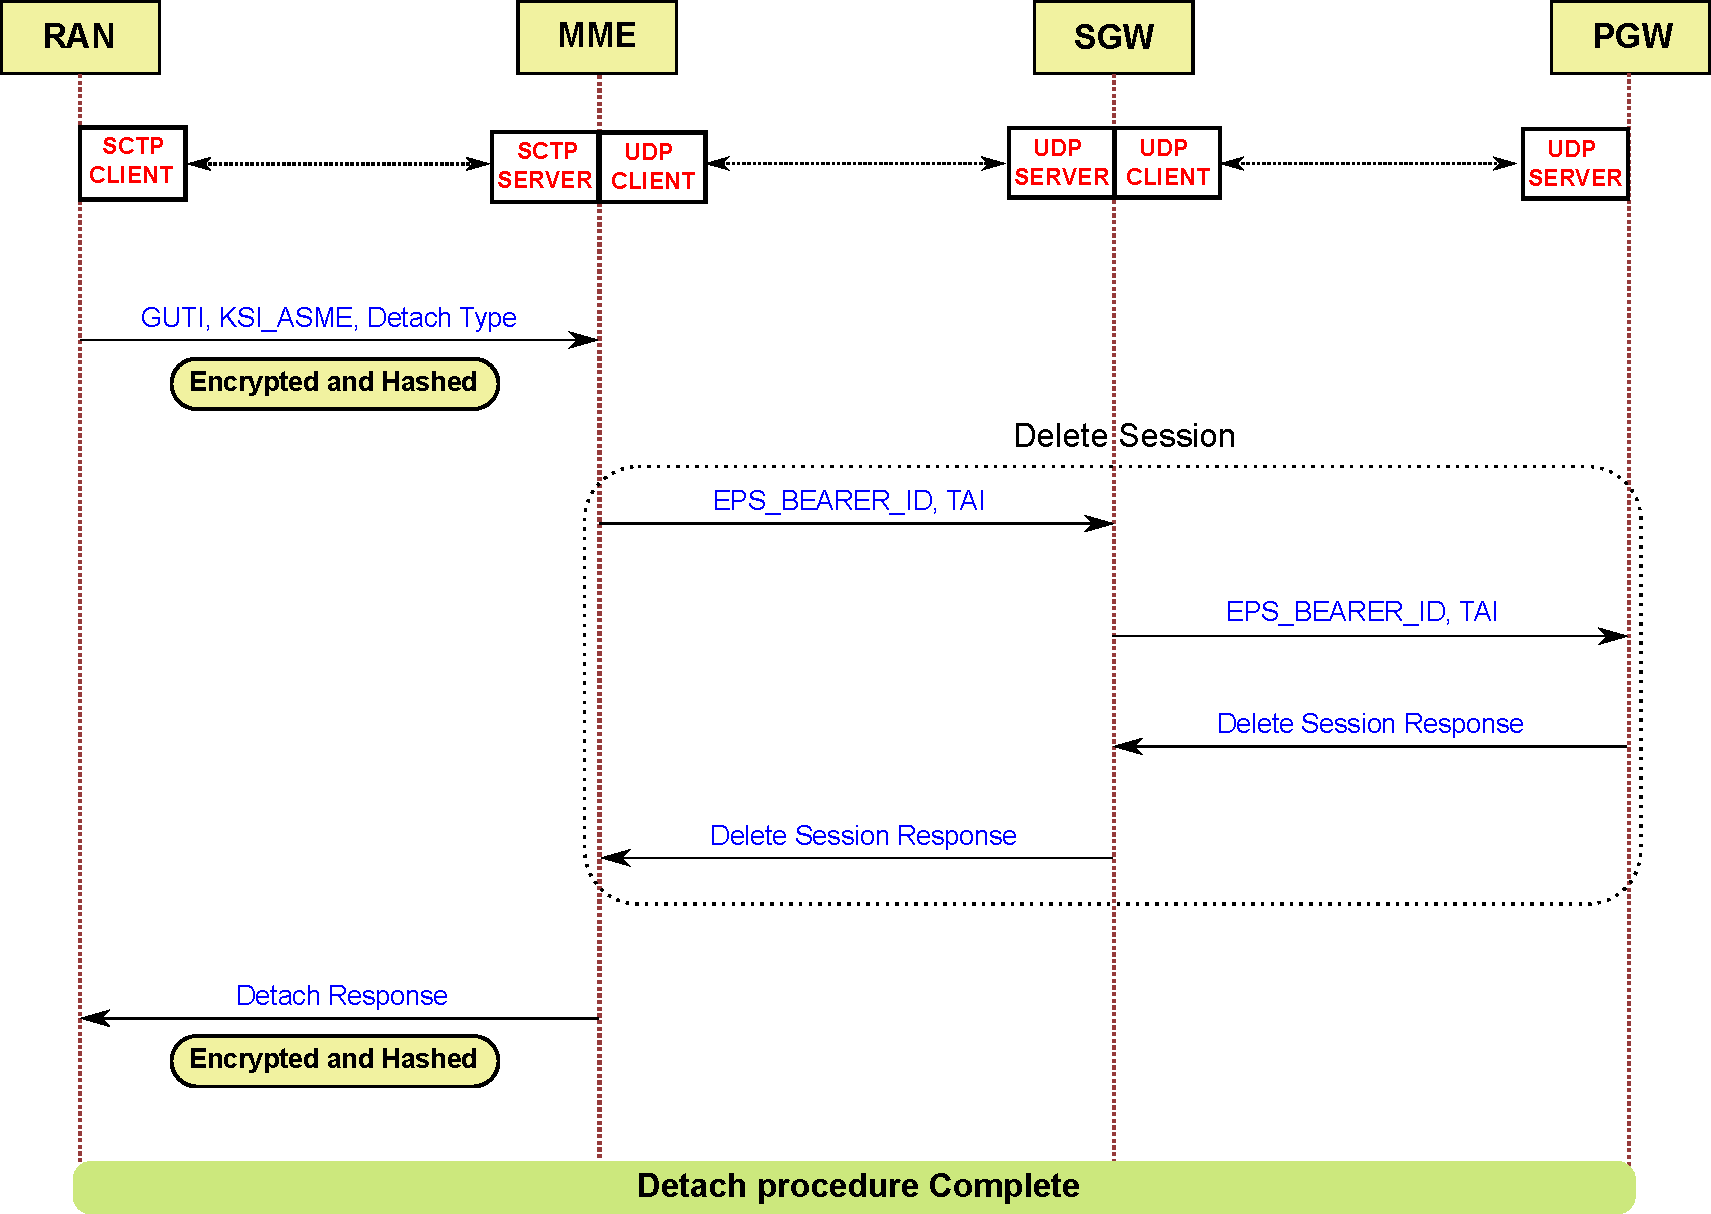
\includegraphics[scale=0.5]{nfv_detach}
\caption{Detach Implementation.}
\label{nfv_detach}

\end{figure}

\begin{enumerate}

\item The UE sends the detach request to the MME.

\item On receiving the detach request, the MME  initiates the delete session procedure with SGW by sending a delete session request.

\item The SGW forwards the request to PGW and on successful detach, success response is propagated from PGW to MME through SGW. The context stored for this UE is removed at all entities.

\item Finally the MME sends the detach response to the UE.

\end{enumerate}

\begin{center}

\subsection*{PART-2 \\ Source Code Overview}

\end{center}

\paragraph*{} In this part, we describe each of the source code files (\cf{.cpp/.h}), and the various functions involved in it. For instance, description about \cf{mme.cpp} and \cf{mme.h} files are given under the section MME.

\subsection*{DIAMETER}

\paragraph*{Description}

~\\ Used for creating a dummy header for \textbf{Diameter} protocol. Employed during communication between MME and HSS. Implemented functions are straightforward to understand.

\subsection*{GTP}

\paragraph*{Description}

~\\ Used for creating a standard header for \textbf{GTP-C} and \textbf{GTP-U} protocols. Employed during tunnel setup and data transfer among MME, SGW, PGW and eNodeB. Implemented functions are straightforward to understand.

\subsection*{HSS}

\paragraph*{Description}

~\\ Employed by \textbf{HSS\_SERVER} in serving requests from the MME module.  Contains various functions that use \textbf{MYSQL} object to communicate with the database. A lock is used around the \textbf{MYSQL} object to prevent data race that might occur because of multithreaded nature of serving requests.

\subsection*{HSS\_SERVER}

\paragraph*{Description}

~\\ Main function for the HSS module. It handles all requests from the MME module and uses a global \textbf{HSS} object to fetch and process required data. Implemented functions initialize necessary parameters and start the server for handling client connections. 

\subsection*{MME}

\paragraph*{Description}

~\\ Contains necessary data structures for storing UE context and MME related information. Implements various functions that deal with UE Session/Bearer creation and termination. It also has a data structure to map S1AP ids to UE GUTI. All global data structures are locked around mutexes for protection.

\subsection*{MME\_SERVER}

\paragraph*{Description}

~\\ Main function for the MME module. It handles all requests from the eNodeBs and uses a global \textbf{MME} object to perform various LTE procedures. Implemented functions initialize necessary parameters and start the server for handling client connections. It also has a set of \textbf{HSS} and \textbf{SGW} client objects, each used in a separate worker thread.

\subsection*{MYSQL}

\paragraph*{Description}

~\\ Responsible for making connection with MySQL database. Stores the connection information (server, user, password, db\_name) and employs a MySQL connection file descriptor to establish DB connection and fetch information. The implemented functions are called by \textbf{HSS} object to satisty various MME requests.

\subsection*{NETWORK}

\paragraph*{Description}

~\\ Contains frequently used functions for socket programming. The implemented functions receive various input parameters along with a socket file descriptor and perform related functions on the received socket file descriptor. A few functions are explained below for clarity.

\begin{itemize}

\item \textbf{func write\_sctp\_packet} Used for sending a SCTP packet. Length of the data is attached along with the data and then written on the socket. This is done to correctly read a SCTP packet at the receiver side, irrespective of whether the sent data gets split into many packets or merged with subsequent data.

\item \textbf{func read\_sctp\_packet} Used for receiving a SCTP packet. While reading, always an integer size of data is read first. This initial data gives the length of the actual data to be read, so that the \cf{read} call can block until the entire packet is received.

\end{itemize}

\subsection*{PACKET}

\paragraph*{Description}

~\\ A template for generating packets. Each \textbf{PACKET} object denotes a packet, where \cf{len} denotes the size of the data in the packet and \cf{data\_ptr} denotes the last index position of the packet. The parameter \cf{data\_ptr} will be helpful while adding/reading/removing the packet data. It contains various functions to modify the packet contents. Some of them are explained below. All such functions modify the length and last index position of the packet data. It also contains functions related to packet headers such as allocating memory for IP headers.

\begin{itemize}

\item \textbf{func append\_item} Insert the input parameter at the end of the packet data. 

\item \textbf{func prepend\_item} Insert the input parameter at the beginning of the packet data.

\item \textbf{func extract\_item} Read the packet data from the last index position into the input parameter supplied. The size of the input parameter is used to decide the length of the packet data that needs to be read.

\item \textbf{func truncate} Copy the packet data from the last index position upto the packet length into a new packet data array. This essentially removes all data that has been extracted before.

\end{itemize}

\subsection*{PGW}

\paragraph*{Description}

~\\ Contains necessary data structure for storing UE context. Implements various functions that deal with the UE Session/Bearer and data transfer. It also has a data structure to map TEIDs to UE IMSI. All global data structures are locked around mutexes for protection. It also implements function to set static IP addresses for UEs.

\subsection*{PGW\_SERVER}

\paragraph*{Description}

~\\ Main function for the PGW module. It handles all requests from the SGW and uses a global \textbf{PGW} object to perform various LTE procedures. Implemented functions initialize necessary parameters and start the servers on S5 and SGi interface ports for handling client connections.

\subsection*{RAN}

\paragraph*{Description}

~\\ RAN module stores RAN contexts of various objects. It implements functions for various EPS Bearer/Session related procedures and uplink/downlink data transfer. It has a separate \textbf{TrafficMonitor} class that deals with packets that need to be sent to/received from the TUN device.

\subsection*{RAN\_SIMULATOR}

\paragraph*{Description}

~\\ Main function for the RAN module. It creates multiple RAN objects for generating control traffic and traffic monitoring objects for handling user plane packets. Employs the functions implemented in \textbf{RAN} to send requests/data transfer. Also responsible for computing various performance metrics for control traffic and data traffic experimentation.

\subsection*{S1AP}

\paragraph*{Description}

~\\ Used for creating a dummy header for \textbf{S1AP} protocol. Employed for communication between MME and eNodeB. Implemented functions are straightforward to understand.

\subsection*{SCTP\_CLIENT}

\paragraph*{Description}

~\\ A simple stream oriented client program that has functions for connecting to a server, sending and receiving SCTP packets. 

\subsection*{SCTP\_SERVER}

\paragraph*{Description}

~\\ Implements the SCTP server architecture described in Part-1. Uses a vector of pipe file descriptors for communication between main acceptor thread and worker threads. Receives the worker thread function as an input parameter, so that client requests can be handled by the remote function present in the module that employs \textbf{SCTPServer} object.

\subsection*{SECURITY}

\paragraph*{Description}

~\\ Contains classes for encryption and integrity check. Both uses the built-in functions of openssl that perform encryption, decryption and HMAC digest generation. AES 256 CBC algorithm is used for encryption/decryption and EVP SHA1 algorithm is used for integrity check. Sample \cf{key} and \cf{iv} values are used for all algorithms; Implemented functions are straightforward to understand.

\subsection*{SGW}

\paragraph{Description}

~\\ Contains necessary data structure for storing UE context. Implements various functions that deal with the UE Session/Bearer and data transfer. It also has a data structure to map TEIDs to UE IMSI. All global data structures are locked around mutexes for protection.

\subsection*{SGW\_SERVER}

\paragraph*{Description}

~\\ Main function for the SGW module. It handles all requests from MME and PGW; uses a global \textbf{SGW} object to perform various LTE procedures. Implemented functions initialize necessary parameters and start the servers on S11, S1 and S5 interface ports for handling client connections.

\subsection*{SINK}

\paragraph*{Description}

~\\ Mainly involved in forwarding traffic between PGW and TUN device. Uses \textbf{UdpServer} and \textbf{Tun} objects.

\subsection*{SINK\_SERVER}

\paragraph*{Description}

~\\ Main function for the Sink module. It has a global \textbf{TrafficMonitor} object from \textbf{SINK} for handling TUN and PDN server (\cf{iperf3}) traffic; creates several threads for running corresponding PDN server objects.

\subsection*{SYNC}

\paragraph*{Description}

~\\ Contains \cf{pthread} functions for initializing mutex, locking/unlocking mutex and wait/signal on mutex. Implemented functions are straightforward to understand.

\subsection*{TELECOM}

\paragraph*{Description}

~\\ Contains functions for computing various telecom parameters such as IMSI and MME Identifier (MMEI). Standard pattern is used for computing all parameters.

\subsection*{TUN}

\paragraph*{Description}

~\\ A simple TUN program that has functions for various TUN related procedures. These procedures include creating a TUN device, attaching to a TUN device, sending/receiving data on a TUN device.

\subsection*{UDP\_CLIENT}

\paragraph*{Description}

~\\ A simple packet oriented client program that has functions for connecting to a server, sending and receiving UDP packets. 

\subsection*{UDP\_SERVER}

\paragraph*{Description}

~\\ Implements the UDP server architecture described in Part-1. Uses a global connection file descriptor \cf{conn\_fd} and manages handling all client requests.

\subsection*{UTILS}

\paragraph*{Description}

~\\ A common program employed by all the modules. Contains most frequently used functions such as error checking and allocating memory.

\end{document}